\chapter{Experiment setup}
Building upon the theoretical framework established in the previous chapter, this chapter introduces the experimental environment used to validate and explore fault-based attacks on SoC interconnects. The structured classification and modeling of vulnerabilities serve as a foundation for the practical investigation that follows. Here, we present the concrete system setup developed to test communication bus security under controlled fault conditions. Specifically, we describe the SoC architecture implemented using the LiteX framework, explain the configuration of the target bus protocols, and define the fault models and attacker assumptions adopted in our study. In addition, we outline the benchmarks and evaluation criteria used to assess the system’s resilience and the effectiveness of potential countermeasures.

\section{Construction SoC}
In order to systematically study fault injection attacks targeting on-chip buses, it is necessary to construct custom SoC platforms where the internal architecture—including interconnects, memory hierarchies, and processor interfaces—can be precisely controlled. This level of flexibility is difficult to achieve using vendor-locked design environments or pre-built SoC platforms, which often lack transparency and configurability at the system level.

To meet these requirements, we chose the LiteX framework. LiteX provides fine-grained control over system configuration, allowing us to tailor bus protocols, memory layouts, and peripheral mappings to suit specific attack scenarios. Moreover, its compatibility with a wide range of FPGA boards ensures that experiments can be reproduced across different hardware targets without extensive redesign. The framework also supports both simulation and hardware deployment from a unified design space, enabling efficient prototyping and testing of attack models.

In the following section, we provide a detailed overview of the LiteX architecture and explain how its features support our experimental goals.
\subsection{LiteX}
The increasing availability of open-source hardware development tools has significantly improved the accessibility and reproducibility of system-on-chip (SoC) research. Among these tools, LiteX (Figure \ref{litex}) has emerged as a versatile and powerful SoC builder framework, designed to streamline the process of constructing FPGA-based systems. Developed by the EnjoyDigital community, LiteX leverages the flexibility of Python and provides a modular and extensible platform for designing, simulating, and deploying digital systems with a high degree of customization.

\begin{figure}[t!]
  \centering
  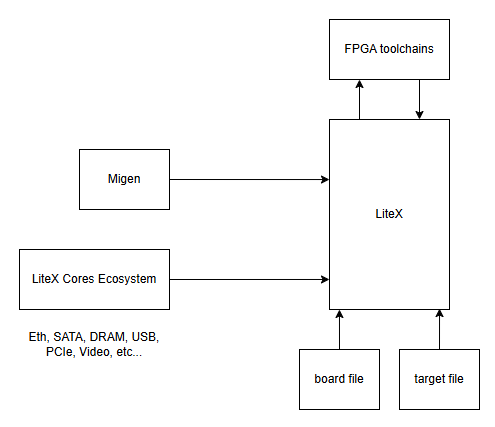
\includegraphics[width=0.5\linewidth]{Chapitre2/figures/litex.png}
  \caption{Component of LiteX framework}
  \label{litex}
\end{figure}

LiteX \cite{litex} provides a comprehensive set of pre-integrated building blocks essential for SoC development. This includes support for common bus protocols and streaming interfaces—such as Wishbone, AXI, and Avalon-ST—along with their corresponding interconnect infrastructure. Core components such as RAM, ROM, UARTs, timers, and JTAG interfaces are readily available, while more sophisticated IP cores—including LiteDRAM, LitePCIe, LiteEth, and LiteSATA—are seamlessly integrated into the ecosystem. The framework supports a variety of CPU architectures and instruction sets, such as RISC-V (e.g., VexRiscv), OpenRISC, LM32, and even x86 (via PCIe integration), enabling both lightweight microcontroller-class SoCs and more complex, Linux-capable multicore systems.

One of the key enablers behind LiteX's flexibility is its foundation in Migen (short for Milkymist generator), a Python-based hardware description library designed to overcome the inefficiencies and limitations of traditional HDLs like Verilog and VHDL. Migen replaces the event-driven model with explicit combinatorial and synchronous constructs, simplifies arithmetic semantics to better reflect mathematical expectations, and, most importantly, allows for procedural generation of logic using standard Python features. This metaprogramming capability empowers developers to write reusable, parameterized, and highly structured hardware designs by leveraging object-oriented patterns, operator overloading, Python generators, and more.

Through the combination of Migen and LiteX, designers benefit from an ecosystem that supports multiple languages (including VHDL, Verilog, SpinalHDL, and nMigen), offers built-in simulation via Verilator for fast and accurate modeling, and includes powerful debugging tools such as Litescope and software bridges for real-time analysis. Furthermore, LiteX supports multiple backend flows, including both open-source and vendor-specific toolchains, enhancing portability and deployment flexibility.

Despite these capabilities, LiteX does not explicitly address security concerns in its architectural design or development workflows. Its primary focus remains on flexibility, modularity, and ease of integration across diverse hardware platforms. This lack of built-in security mechanisms—such as privilege enforcement, fault injection resistance, or hardware isolation—makes it a particularly interesting target for security research. Given its increasing adoption in research and prototyping contexts, analyzing LiteX from a security perspective is not only timely but essential. Investigating its behavior under adversarial conditions can help identify architectural gaps and motivate the development of lightweight, security-enhanced extensions suitable for resource-constrained environments.

In this research, we adopt LiteX as the foundation for constructing various SoC instances that serve as testbeds for our fault injection experiments. The platform enables the controlled configuration of interconnects (e.g., Wishbone vs AXI-Lite), memory subsystems, and processor types, facilitating detailed comparisons across different architectural choices. The ability to instrument hardware, modify firmware, and run cycle-accurate simulations within a unified development environment makes LiteX particularly well-suited for studying software-assisted fault attacks. Notably, complex SoCs—such as a multicore Linux-capable system based on VexRiscv-SMP, LiteDRAM, and LiteSATA—can be assembled, tested, and deployed using LiteX, even on cost-effective FPGA platforms.

\subsection{SoC configuration}
As we talk before, we designed a highly customizable and transparent system-on-chip (SoC) platform to support controlled experimentation of fault injection attacks targeting interconnect-level vulnerabilities. This platform was implemented using the LiteX framework, which enables fine-grained architectural control and streamlined deployment on FPGA hardware. Each component of the SoC—from the processor core to the interconnects and memory subsystem—was carefully selected to facilitate precise observation, fault reproducibility, and architectural flexibility across experimental scenarios.

At the heart of the system is the VexRiscv soft-core CPU, an open-source implementation of the RISC-V instruction set. We selected RISC-V for its minimalistic and modular architecture, which simplifies reasoning about instruction-level behavior during fault injection. The open specification of RISC-V provides complete transparency over instruction decoding, execution semantics, and control paths—properties essential for correlating fault effects with specific hardware events. VexRiscv’s configurability, small footprint, and close integration with the LiteX ecosystem make it ideal for deploying on resource-constrained FPGA platforms while maintaining the option to scale up with more advanced features. Furthermore, VexRiscv’s support for real-time debugging and visibility into register-level state significantly aids in fault localization.

To analyze the impact of bus-level faults in varied contexts, we designed the SoC to support three major interconnect protocols: Wishbone, AXI, and AXI-Lite. These buses differ in complexity and transaction semantics, offering diverse opportunities for observing different classes of fault behavior. Wishbone, as a synchronous and minimal protocol, is easy to analyze and useful for capturing fundamental fault patterns. In contrast, AXI introduces advanced features such as out-of-order execution, burst transfers, and independent read/write channels, thereby increasing the range and subtlety of observable vulnerabilities. AXI-Lite, a subset of AXI without burst or outstanding transaction support, serves as a middle ground—maintaining AMBA compatibility while retaining relatively simple timing. By keeping the rest of the SoC architecture constant, we can isolate the impact of the bus protocol itself when assessing system-level fault behavior.

The memory architecture of the SoC includes four primary regions: ROM, SRAM, CSR (Control and Status Registers), and an additional MAIN\_RAM block. The ROM is used to store program binaries and is loaded at synthesis time. To ensure maximal control over program behavior, all software is compiled into unoptimized assembly using the RISC-V GCC toolchain with -O0 optimization level. This prevents the compiler from reordering instructions or introducing artifacts that could obscure fault propagation paths. By using hand-tuned or compiler-generated low-level code, we achieve consistency across test cases and precise mapping between source and hardware behavior.

SRAM is used as the main runtime memory for variables, stack, and temporary data. The CSR region is memory-mapped and provides access to internal system signals such as timers, bus status, and control flags. These are particularly useful for monitoring injected fault effects from within the program itself. To further extend our experimental capabilities, we introduced an additional MAIN\_RAM region. This memory block is configured to behave identically to the SRAM—sharing the same address decoding logic and latency characteristics. By duplicating memory structures, we can construct controlled experiments that differentiate between location-based fault effects and memory controller behavior, as well as explore dual-memory scenarios such as DMA transfers or mirrored execution contexts.

The entire system is synthesized and deployable on the Digilent Basys3 FPGA development board, which features a Xilinx Artix-7 (XC7A35T) device. This board offers a balanced trade-off between accessibility and capability, and is well-supported by the LiteX framework as well as both open-source (Yosys, nextpnr) and vendor-specific toolchains. While physical deployment is possible, our fault injection methodology is conducted entirely in simulation, leveraging the built-in Verilator backend provided by LiteX. This simulation-based approach allows for fine-grained control over timing and internal signal states without requiring physical probes or glitch hardware.

The Basys3 platform is still relevant in this context: it defines the target architecture for the simulation, ensuring that resource constraints (e.g., logic and memory limits) are realistic and that timing behavior remains consistent with actual FPGA implementations. The board’s well-documented peripherals and standard clocking scheme also serve as a reference for cycle-accurate modeling during simulation. Furthermore, its affordability and broad availability support future hardware validation or replication, should post-simulation testing be desired.

Software execution on this platform begins from the ROM, with the program executing directly from its binary image. When needed, specialized boot code is used to copy program segments into writable memory areas such as SRAM or MAIN\_RAM. The lack of virtual memory and the flat address layout reduce complexity and ensure that observed effects are directly attributable to hardware behavior, rather than memory management artifacts.

Together, this SoC configuration provides a controlled, transparent, and reproducible environment for evaluating the impact of fault injection on communication buses and related subsystems. The use of a unified hardware/software stack, fine-tuned for experimentation, allows us to isolate fault origins, track propagation paths, and assess the robustness of interconnects under various attack conditions.

\section{Fault model}

\subsection{benchmark}

To investigate and exploit the effects of fault injection, we established a comprehensive test environment utilizing the well-known VerifyPin benchmark suite. Developed in C as part of the Sertif project~\cite{dureuil2016fissc}, VerifyPin comprises eight implementations: one unprotected baseline (V0) and seven protected variants (V1 through V7), each integrating different countermeasures against previously described software attacks. For each experimental run, one version of VerifyPin is embedded in the SoC’s ROM. While the following chapter details the seven countermeasures, here we introduce the program structure and functionality using V0 as a representative example.

VerifyPin version 0 is a lightweight, standalone C program simulating a secure PIN verification process. It is designed to evaluate security vulnerabilities and fault injection impacts on embedded systems by realistically modeling critical security code behaviors through a combination of control flow, memory operations, and optional protection features. The benchmark employs a modular software architecture composed of multiple source and header files, each responsible for specific functions to ensure maintainability and facilitate targeted testing. Except for the code.c file, all other files remain consistent across different versions.

Figure~\ref{fig:file-tree} illustrates the hierarchical file dependency structure of the VerifyPin version 0. At the core lies \texttt{main.c}, which acts as the central coordination unit and integrates multiple components, including headers such as \texttt{interface.h}, \texttt{types.h}, and \texttt{lazart.h}, as well as key source files like \texttt{initialize.c}, \texttt{code.c}, and \texttt{oracle.c}. Among these, \texttt{code.c} introduces a secondary layer of dependency by incorporating \texttt{common.h} and \texttt{countermeasure.h}, reflecting a modular design that separates core logic from reusable definitions and countermeasure strategies. This structured organization simplifies simulation-based fault injection experiments by enabling targeted instrumentation of individual modules.

\begin{figure}
    \centering
    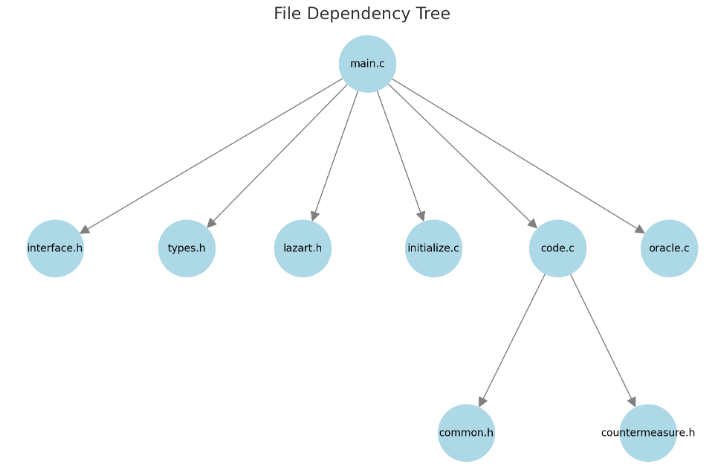
\includegraphics[width=0.75\linewidth]{Chapitre2/figures/tree.png}
    \caption{File dependency structure of the project. }
    \label{fig:file-tree}
\end{figure}

The program’s entry point resides in main.c in Listing\ref{main}, which handles system initialization(line 14), obtains user input—either simulated or fault-injected—and invokes the PIN validation logic(line 15) contained within the oracle module(line 16). The main function further processes the verification outcome and provides appropriate feedback(line 18 to 19). This file exemplifies typical control flow in embedded applications and is instrumental in assessing the resilience of entry and decision points under fault conditions.
\begin{figure}
\begin{lstlisting}[caption={main.c of VerifyPin function in benchmark V0}, label={main}, basicstyle=\ttfamily\footnotesize]
#include <stdio.h>
#include "interface.h"
#include "types.h"
#include "lazart.h"

extern UBYTE g_countermeasure;
extern BOOL g_authenticated;
extern SBYTE g_ptc;

BOOL verifyPIN(void);

int main()
{
    initialize();
    verifyPIN();
    LAZART_ORACLE(oracle());
    
    printf("[@] g_countermeasure = %i, g_authenticated = %x, g_ptc = %i\n", g_countermeasure, g_authenticated, g_ptc);
    return 0;
}
\end{lstlisting}
\end{figure}
The core decision-making logic is implemented in oracle.c in Listing\ref{oracle}, which performs a byte-wise comparison between the user-supplied PIN and the stored correct value. This approach mimics early-exit behaviors found in real-world implementations, offering exploitable points for differential fault analysis and side-channel attacks. The oracle deliberately omits certain protections such as masking or constant-time operations, making it a key target for both software- and hardware-based fault injections.
\begin{figure}
\begin{lstlisting}[caption={oracle.c of VerifyPin function in benchmark V0}, label={oracle}, basicstyle=\ttfamily\footnotesize]
#include "interface.h"
#include "types.h"

#ifdef AUTH
#define oracle_auth oracle
#endif

#ifdef PTC
#define oracle_ptc oracle
#endif

extern UBYTE g_countermeasure;
extern BOOL  g_authenticated;
extern SBYTE g_ptc;

BOOL oracle_auth()
{
    return g_countermeasure != 1 && g_authenticated == 1;
}

BOOL oracle_ptc()
{
    return g_countermeasure != 1 && g_ptc >= 3;
}
\end{lstlisting}
\end{figure}
Supporting utility functions are implemented in \texttt{code.c} (Figure~\ref{code}), including routines for memory comparison, data copying, and buffer manipulation. Although these functions are not directly exposed through external interfaces, they play a crucial role in shaping the program’s internal behavior and attack surface. Improper handling of memory within these helpers can introduce vulnerabilities, making them potential vectors for memory corruption attacks. Moreover, since these routines are reused across all benchmark versions, their correctness and security are essential for consistent evaluation and meaningful fault injection results.

To illustrate the core logic of the benchmark, we use version V0 as a representative example (Listing~\ref{code}). In this version, the program compares the user-entered PIN, stored in the variable \texttt{g\_userPin} (initialized to \texttt{"0000"}), with the correct card PIN, stored in \texttt{g\_cardPin} (initialized to \texttt{"4321"}). The PIN comparison logic simulates typical authentication behavior in embedded applications(line 29). Under normal conditions, the PINs do not match, and the program sets the \texttt{g\_authenticated} flag to \texttt{0}, indicating authentication failure(line 35). A successful fault injection attack can be detected when \texttt{g\_authenticated} is erroneously set to \texttt{1} despite the mismatch(line 31). The use of 0000 as the user input ensures a consistent and minimal binary pattern (all zeros), simplifying fault localization and enabling clear observation of bit flips or instruction corruption during the attack. Meanwhile, setting the card PIN to 4321 introduces a nontrivial comparison target with varied bit transitions, enhancing the likelihood of detecting successful bypasses or erroneous matches induced by injected faults. This contrast between the two values allows for precise control and clearer differentiation between correct and faulty program behavior in our analysis.

The number of permitted authentication attempts is managed by the variable \texttt{g\_ptc}, which is initialized to \texttt{3} and decremented after each failed attempt. Once \texttt{g\_ptc} reaches zero, further login attempts are blocked, simulating a basic protection against brute-force attacks. In the protected benchmark versions (V1 to V7), an additional countermeasure mechanism is introduced: when a fault is detected, a dedicated routine sets the variable \texttt{g\_countermeasure} to \texttt{1}. This mechanism enables the evaluation of the benchmark’s response to fault injection attempts, providing a clear indicator of whether the protection logic has correctly identified and responded to anomalous behavior.
\begin{figure}
\begin{lstlisting}[caption={code.c of VerifyPin function in benchmark V0}, label={code}, basicstyle=\ttfamily\footnotesize]
#include "interface.h"
#include "types.h"
#include "commons.h"

extern SBYTE g_ptc;
extern BOOL g_authenticated;
extern UBYTE g_userPin[PIN_SIZE];
extern UBYTE g_cardPin[PIN_SIZE];

#ifdef INLINE
__attribute__((always_inline)) inline BOOL byteArrayCompare(UBYTE* a1, UBYTE* a2, UBYTE size)
#else
BOOL byteArrayCompare(UBYTE* a1, UBYTE* a2, UBYTE size)
#endif
{
    int i;
    for(i = 0; i < size; i++) {
        if(a1[i] != a2[i]) {
            return 0;
        }
    }
    return 1;
}

BOOL verifyPIN() {
    g_authenticated = 0;

    if(g_ptc > 0) {
        if(byteArrayCompare(g_userPin, g_cardPin, PIN_SIZE) == 1) {
            g_ptc = 3;
            g_authenticated = 1; // Authentication();
            return 1;
        } else {
            g_ptc--;
            return 0;
        }
    }

    return 0;
}
\end{lstlisting}
\end{figure}
The initialization logic in initialize.c in Listing\ref{initialize} configures the program’s starting state by setting up internal data structures, initializing the correct PIN, and preparing buffers for interaction between the oracle and main program(line 21 to 28). This module ensures experiment reproducibility and consistency. Faults injected at this stage may induce persistent corruptions, making initialization a sensitive phase for certain attack types.
\begin{figure}
\begin{lstlisting}[caption={initialize.c of VerifyPin function in benchmark V0}, label={initialize}, basicstyle=\ttfamily\footnotesize]
#include "types.h"
#include "interface.h"
#include "commons.h"

// global variables definition
BOOL g_authenticated;
SBYTE g_ptc;
UBYTE g_countermeasure;
UBYTE g_userPin[PIN_SIZE];
UBYTE g_cardPin[PIN_SIZE];


void initialize()
{
   // local variables
   int i;
   // global variables initialization
   g_authenticated = 0;
   g_ptc = 3;
   g_countermeasure = 0;
   // card PIN = 1 2 3 4 5...
   for (i = 0; i < PIN_SIZE; ++i) {
       g_cardPin[i] = i+1;
   }
   // user PIN = 0 0 0 0 0...
   for (i = 0 ; i < PIN_SIZE; ++i) {
       g_userPin[i] = 0;
   }
}
\end{lstlisting}
\end{figure}
Basic protective features are implemented in countermeasure.c in Listing\ref{countermeasure}, simulating lightweight security mechanisms common in embedded applications. These include redundancy checks, sanity validations, and simple tamper detection routines. Though not exhaustive or production-grade, these countermeasures increase the complexity of the program’s state space and control flow, facilitating evaluation of attack strategies and security-performance trade-offs.
\begin{figure}
\begin{lstlisting}[caption={countermeasure.c of VerifyPin function in benchmark V0}, label={countermeasure}, basicstyle=\ttfamily\footnotesize]
#include "interface.h"
#include "types.h"

extern UBYTE g_countermeasure;

void countermeasure()
{
    g_countermeasure = 1;
}
\end{lstlisting}
\end{figure}
Types used throughout the benchmark, such as fixed-width integers (u8, u16, u32), are defined in types.h in Listing\ref{types}, promoting portability and deterministic behavior across platforms. This ensures consistent execution on both 32-bit and 64-bit systems, easing deployment in various simulation and hardware environments.
\begin{figure}
\begin{lstlisting}[caption={types.c of VerifyPin function in benchmark V0}, label={types}, basicstyle=\ttfamily\footnotesize]
#ifndef H_TYPES
#define H_TYPES
typedef signed char   SBYTE;
typedef unsigned char UBYTE;
typedef unsigned char BOOL;
typedef unsigned long ULONG;

#define BOOL_TRUE 0xAA
#define BOOL_FALSE 0x55

#endif // H_TYPES
\end{lstlisting}
\end{figure}
The interface between the core logic and external components is defined in interface.h, as shown in Listing~\ref{interface}. This header file specifies function prototypes and outlines the expected input/output data structures. It encapsulates the declarations of key functions, including the countermeasure, initialization, and oracle routines.
\begin{figure}
\begin{lstlisting}[caption={interface.h of VerifyPin function in benchmark V0}, label={interface}, basicstyle=\ttfamily\footnotesize]
#ifndef H_INTERFACE
#define H_INTERFACE

#include "types.h"

/* defines what happens when a fault has been detected
    implementation defined
*/
void countermeasure(void);

/* initializes global variables at the beginning of an example
    implementation-defined
    example-defined
*/
void initialize(void);

/* determines whether an attack is successful
    example-defined
*/
BOOL oracle(void);

#endif // H_INTERFACE
\end{lstlisting}
\end{figure}
Configuration options and compile-time toggles are centralized in lazart.h in Listing\ref{lazart} through macros controlling features such as debug printing, countermeasure activation, and early-return behavior. This allows flexible customization without altering the core code, enabling researchers to adjust program complexity and security levels for different test scenarios.
\begin{figure}
\begin{lstlisting}[caption={lazart.c of VerifyPin function in benchmark V0}, label={lazart}, basicstyle=\ttfamily\footnotesize]
#ifndef LAZART_API_HPP
#define LAZART_API_HPP

#ifdef LAZART

#include <klee/klee.h>

/*#define LAZART_ORACLE(oracle)               \
    if(oracle) {                            \
        klee_assume(oracle);                \
    } else {                                \
        klee_assume(0 != 0 );               \
    }*/

#define LAZART_ORACLE(oracle) klee_assume(oracle)

#else
#define LAZART_ORACLE(oracle)
#endif // LAZART

#endif // LAZART_API_HPP
\end{lstlisting}
\end{figure}
Shared constants, macros, and common includes are consolidated in commons.h in Listing\ref{commons} to improve maintainability and maintain consistency across files. This header typically contains global variables, debug settings, and high-level parameters, embodying best coding practices critical for modularity and clarity in embedded system development.
\begin{figure}
\begin{lstlisting}[caption={commons.c of VerifyPin function in benchmark V0}, label={commons}, basicstyle=\ttfamily\footnotesize]
#ifndef H_COMMONS
#define H_COMMONS

// macro definitions
#define INITIAL_VALUE 0x2a
#define PIN_SIZE 4

#endif // H_COMMONS
\end{lstlisting}
\end{figure}
In summary, VerifyPin V0 presents a compact yet comprehensive foundation for embedded software security analysis. The distinct roles of each source file—from user input handling and data verification to countermeasure implementation and configuration management—enable precise attack simulation, reproducibility, and adaptability. By exposing critical control and data flows, this benchmark serves as an effective tool for evaluating fault injection effects, validating detection mechanisms, and deepening the understanding of software vulnerabilities within constrained embedded environments.

\subsection{FISSA}
To efficiently handle the large number of simulations required for a comprehensive evaluation of the architecture's robustness, we employed FISSA (Fault Injection Simulation for Security Assessment)~\cite{PLG-24-dsd}, a Python-based tool specifically developed for generating and managing fault injection campaigns targeting microarchitectures. FISSA is designed to operate in conjunction with standard HDL simulators such as Questasim, Vivado, or Verilator, enabling users to conduct fault injection experiments within the same environment used for functional design and verification. This seamless integration supports both the validation of design functionality and the assessment of its resilience against physical fault injection attacks (FIA), thereby facilitating the development of effective countermeasures. In our work, we adopt the tool using the Questasim simulation backend and present the corresponding fault injection workflow.In this section, we provide a general introduction. The specific application of FISSA will be discussed in the next chapter.

\begin{figure}[t!]
  \centering
  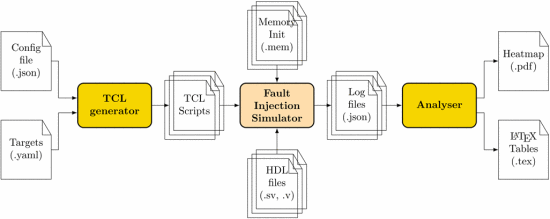
\includegraphics[width=0.5\linewidth]{Chapitre2/figures/fissa.png}
  \caption{FISSA component (source: \cite{PLG-24-dsd})}
  \label{fissa}
\end{figure}

FISSA is composed of three main components(Figure \ref{fissa}): the TCL Generator, the Fault Injection Simulator, and the Analyser. In our experiments, we utilize the first two components. The TCL Generator is responsible for producing the simulation scripts based on the specified configuration and fault parameters, while the Fault Injection Simulator executes these scripts to perform the actual simulations and generate structured log outputs for later analysis.

The TCL script generation process is driven by a set of Python classes, each responsible for producing portions of the final output scripts. The process begins with an initialisation class that extracts parameters from a JSON-formatted configuration file. This file specifies key simulation settings, including the HDL simulator to be used, the fault model, injection window(s), the design’s clock period (in nanoseconds), and the maximum number of simulation cycles allowed before forced termination in case of divergence. It also defines the number of simulations to be included in each TCL file, which determines the degree of parallelism in simulation execution.

In addition to the configuration file, a separate YAML-formatted targets file lists the elements of the circuit to be faulted—such as registers or logic gates—along with their HDL paths and bit-widths. These targets are essential inputs to the fault injection campaign.

Based on the configuration and target data, the TCL Script Generator class coordinates the creation of complete TCL scripts. It delegates specific tasks to three auxiliary classes. The Basic Code Generator produces the core TCL instructions to initialize, run, and terminate a simulation. The Fault Generator creates TCL code that defines fault injection operations, using parameters that specify target elements and fault injection clock cycles. The Log Generator outputs TCL code for automated logging of simulation metadata, including simulation ID, fault model, faulted elements, injection time, status at simulation end, values of all targets, and the final simulation cycle.

Each TCL file corresponds to a batch of simulations and begins with a reference simulation without fault injection. This enables result comparison within each batch. Additionally, a standalone target file is generated for TCL scripts to retrieve the fault injection targets.

The Fault Injection Simulator operates by leveraging an existing HDL simulator, which executes the TCL scripts generated during the previous stage. For each simulation, a corresponding log file is produced in JSON format, capturing essential metadata such as the simulation index, the number of clock cycles executed, the values from the target file, the faulted elements, the applied fault model, and the final simulation status.

To ensure seamless integration within the designer’s existing workflow, the invocation of these TCL scripts must be incorporated into the broader design process. This includes stages such as design compilation, initialization, and input stimulus management. The script-based approach facilitates this integration by providing a modular and automated interface to the simulation environment.

After completing all fault injection campaigns, the resulting log files are passed to the Analyser component, which is introduced in the following subsection.

\subsection{Attack model}

In this study, we define a realistic and constrained fault injection threat model tailored for the evaluation of embedded security mechanisms under simulation. The attacker operates in a black-box setting, with no knowledge of the correct PIN value stored in the system, which is initialized as \texttt{"4321"} in all test cases. The input PIN, set to \texttt{"0000"}, is deliberately incorrect to ensure that any successful authentication outcome can be attributed solely to fault-induced corruption. This assumption reflects practical attack scenarios where the attacker is unable to retrieve or infer secret values through direct observation.

Fault injection is performed within a simulation environment using TCL commands generated by the FISSA tool. These commands emulate physical fault attacks at the register-transfer level (RTL), injecting faults into specific control elements during simulation time. The attack campaign is automated and covers multiple clock cycles corresponding to the execution of the \texttt{verifyPIN} function \ref{code} and the targeting of critical registers, providing a broad view of the system’s vulnerability to transient faults. In order to evaluate the robustness of the architecture under a diverse range of attack scenarios, we also introduced different-level-complexity fault models predefined in FISSA (Figure \ref{fault model}). The considered models are all single-cycle attacks:
\begin{enumerate}
\item Bit-Flip: 1 bit-flip in register.
\item Manipulate Register: This model allows arbitrary bit-flips in any single register. Both the number of flipped bits and their positions within the register are unrestricted, simulating a wide range of fault patterns within a single storage element.
\item 2 Bit-Flips: This model restricts fault injection to exactly two bit-flips. The two flipped bits may occur within the same register or across two different registers. This model is designed to represent dual-bit fault scenarios, such as multi-bit upsets (MBUs) induced by radiation or other environmental factors.
\item Manipulate Two Registers: This model extends the manipulation to two distinct registers, where each register can experience arbitrary numbers of bit-flips at arbitrary positions. This model captures complex fault cases involving simultaneous corruption across multiple storage elements.
\end{enumerate}

\begin{figure}[t!]
  \centering
  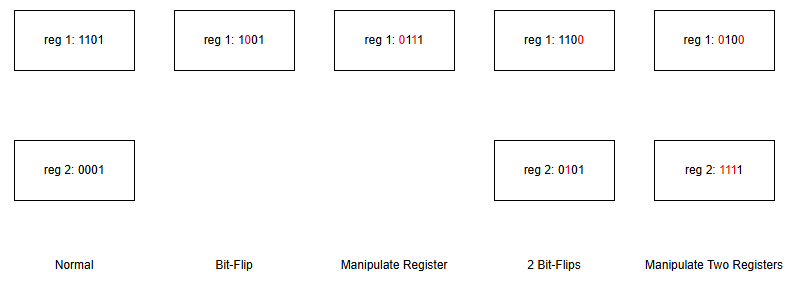
\includegraphics[width=0.5\linewidth]{Chapitre2/figures/fault model.png}
  \caption{Example of 4 fault models}
  \label{fault model}
\end{figure}

According to the article\cite{sass2023oops}, the models are constrained to generate at most four faults, which is deemed adequate for capturing the dominant classes of fault injection behavior observed in practical systems. These diversified fault models enable more comprehensive coverage of possible fault manifestations and allow finer-grained analysis of the architecture’s fault tolerance capabilities.

The scope of the attack is intentionally limited to control registers connected to the system bus, excluding data and address lines. This restriction reflects common architectural protections: in many embedded systems, address and data buses are either not latched in vulnerable registers or are protected through error detection and correction (EDC) mechanisms, such as parity bits or ECC codes. As such, targeting them in fault injection campaigns would either be ineffective or unrepresentative of realistic fault propagation paths. By focusing on control registers—such as status flags, authentication result indicators, or loop counters—we model an attacker capable of subtly influencing the control flow of the software without inducing immediate system crashes or violating low-level bus protocols.

A fault is considered successful if it leads to an unauthorized authentication, i.e., the variable \texttt{g\_authenticated} is incorrectly set to \texttt{1} despite the incorrect input PIN. Importantly, successful faults must not cause the system to halt, crash, or enter undefined behavior states. Furthermore, in protected versions of the benchmark (V1 to V7), any such fault must also evade detection or correction by the implemented countermeasures. To systematically analyze the effects of fault injection, the simulation results were categorized into five distinct outcomes:
\begin{enumerate}
\item Crash, the simulation either exceeded the fixed execution time or triggered a crash signal, resulting in termination.
\item Detect, the fault was detected by the countermeasure, setting the variable \texttt{g\_countermeasure} to "1".
\item Success, the authentication bypassed successfully, with \texttt{g\_authenticated} set to "1".
\item Change, no successful authentication or detection occurred, but the memory state was altered by the fault.
\item Silence, no authentication success, detection, or memory state change was observed, indicating the fault had no visible impact.
\end{enumerate}
Among these, only the “Success” outcome, defined as the achievement of unauthorized authentication without detection or system failure, qualifies as a valid and exploitable fault from an attacker’s perspective.

The system under test incorporates both hardware and software countermeasures. Hardware-level protections may be embedded in the Verilog design of the system, including fault-tolerant state machines or error-detection logic at the bus interface. On the software side, the VerifyPin benchmark provides seven protected implementations (V1–V7), each incorporating a different strategy to detect or tolerate fault effects—ranging from control flow integrity checks to redundant variable encoding.

This threat model allows for controlled and repeatable evaluation of the system’s security posture under targeted, register-level fault injection, providing valuable insight into the effectiveness of different defensive strategies and the residual risks that remain even under constrained attacker capabilities.

\section{Conclusion}
In summary, this chapter has established a comprehensive experimental framework for evaluating fault-based attacks targeting SoC interconnects. By detailing the SoC architecture, bus configurations, attacker model, and fault injection methodology, we have laid the technical groundwork for systematic and reproducible analysis. The integration of configurable benchmarks and clear evaluation metrics further enables meaningful comparisons across different protection strategies and fault scenarios. Building on this foundation, the next chapter delves into the exploitation of vulnerabilities specific to the communication buses under study—namely, Wishbone, AXI-Lite, and AXI—demonstrating how carefully crafted fault injections can compromise data integrity, control flow, and system behavior across these widely-used protocols.
